\special{dvipdfmx:config z 0}
\documentclass[12pt, a4paper, oneside]{ctexbook}
\usepackage{amsmath, amsthm, amssymb, bm, graphicx, hyperref, mathrsfs, float, subfigure, svg, color}
\usepackage{listings}
\usepackage{ctex}

\makeatletter
\newcommand{\rmnum}[1]{\romannumeral #1}
\newcommand{\Rmnum}[1]{\expandafter\@slowromancap\romannumeral #1@}
\makeatother

% 用来设置附录中代码的样式

\lstset{
    basicstyle          =   \sffamily,          % 基本代码风格
    keywordstyle        =   \bfseries,          % 关键字风格
    commentstyle        =   \rmfamily\itshape,  % 注释的风格,斜体
    stringstyle         =   \ttfamily,  % 字符串风格
    flexiblecolumns,                % 别问为什么,加上这个
    numbers             =   left,   % 行号的位置在左边
    showspaces          =   false,  % 是否显示空格,显示了有点乱,所以不现实了
    numberstyle         =   \zihao{-5}\ttfamily,    % 行号的样式,小五号,tt等宽字体
    showstringspaces    =   false,
    captionpos          =   t,      % 这段代码的名字所呈现的位置,t指的是top上面
    frame               =   lrtb,   % 显示边框
}

\lstdefinestyle{Python}{
    language        =   Python, % 语言选Python
    basicstyle      =   \zihao{-5}\ttfamily,
    numberstyle     =   \zihao{-5}\ttfamily,
    keywordstyle    =   \color{blue},
    keywordstyle    =   [2] \color{teal},
    stringstyle     =   \color{magenta},
    commentstyle    =   \color{red}\ttfamily,
    breaklines      =   true,   % 自动换行,建议不要写太长的行
    columns         =   fixed,  % 如果不加这一句,字间距就不固定,很丑,必须加
    basewidth       =   0.5em,
}

\title{{\Huge{\textbf{Chapter1 神经元和数学方法}}}}
\author{黄志权}
\date{\today}
\linespread{1.5}
\newtheorem{theorem}{定理}[section]
\newtheorem{definition}[theorem]{定义}
\newtheorem{lemma}[theorem]{引理}
\newtheorem{corollary}[theorem]{推论}
\newtheorem{example}[theorem]{例}
\newtheorem{proposition}[theorem]{命题}
\CTEXsetup[format={\Large\bfseries}]{section}

\begin{document}

\maketitle

\pagenumbering{roman}
\setcounter{page}{1}

\newpage
\pagenumbering{Roman}
\setcounter{page}{1}
\tableofcontents
\newpage
\setcounter{page}{1}
\pagenumbering{arabic}

\chapter{LIF模型(Leaky-Integrate-and-fire models)}
神经元的动力模型可以被简化为:树突接收若干的脉冲信号,并积累到细胞膜上,致使细胞膜电压改变,从而产生动作电位。LF模型则是将动作电位描述成事件的模型。

\section{膜电压$u(t)$演变的线性微分方程推导}
对于神经元细胞,我们可以将其想象为如下的RC电路。细胞膜就像是一个与电阻并联的电容器,而电阻连接着一个电压为$u_{rest}$电池。当没有外界输入时,膜电压$u(t)$为初始值$u_{rest}$;当有外界脉冲输入时,相当于给电容提供电流为$I(t)$的充电,从而改变模电压$u(t)$。//PS:这个电阻也被称为漏电阻。由于在没有外界输入时,膜上电荷会逐渐穿过细胞膜泄露出去,让膜电压回归$u_{rest}$,因此引入一个漏电阻来模拟这种现象。

\begin{figure}[H]
    \centering
    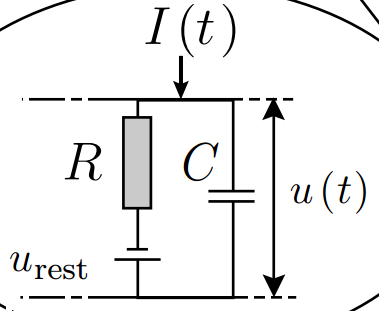
\includegraphics[width=0.3\textwidth]{细胞膜等效电路.png}
    \caption{细胞膜等效电路}
\end{figure} 

考虑$I(t)$不为零的情况,即有外界输入时,来分析膜电压的变化。首先总电流由并联电路支电流和组成$I(t)=I_r+I_C$。即:

\begin{equation}
I(t)=\frac{u(t)-u_{rest}}{R}+C\frac{du(t)}{dt}    
\end{equation}

模仿电路分析,定义膜时间常数(membrane time constant)$\tau _m=RC$。从而可以得到$u(t)$的线性微分方程:

\begin{equation}
    \tau _m\frac{du(t)}{dt}= -[u(t)-u_{rest}] + RI(t)
    \label{微分方程}
\end{equation}

上式在电路分析中称为RC电路响应方程,在神经科学领域称为无源膜方程(equation of a passive membrane)。这个方程的解分为两个部分。即输入脉冲的充电过程(零状态响应),和没有输入脉冲,电压泄露到$u_{rest}$的过程(零状态响应)。首先是输入脉冲的充电过程(零状态响应),我们假设输入电流脉冲在$t_0$时刻是一个幅值为$I_{max}$的方波,则其方程如下:

\begin{equation}
    u(t)=u_{rest}+I_{max}R(1-e^{-\frac{t-t_0}{\tau_m}})
    \label{零状态响应}
\end{equation}

\begin{figure}[H]
    \centering
    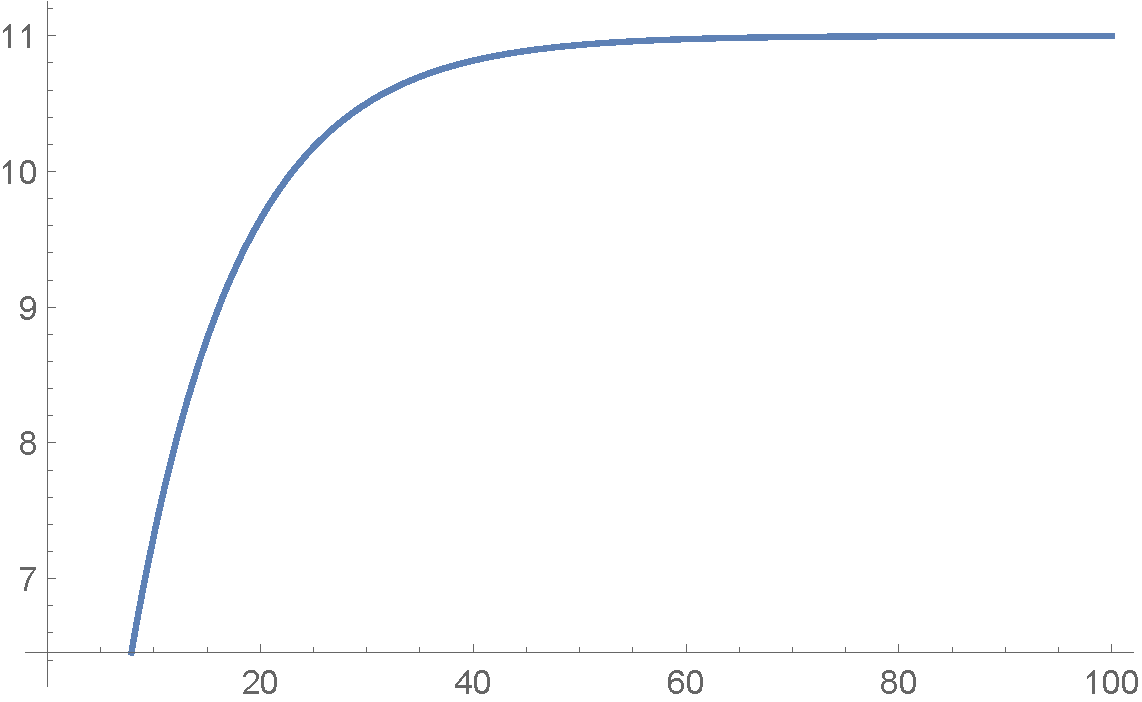
\includegraphics[width=0.5\textwidth]{脉冲充电图.pdf}
    \caption{脉冲充电图}
\end{figure} 

然后是电压泄露到$u_{rest}$的过程(零状态响应),假设脉冲在$t_1$时刻结束:

\begin{equation}
    \begin{aligned}
        u(t)&=u_{rest}+\Delta u Re^{-\frac{t-t_1}{\tau_m}}\\ \Delta u&=u(0)-u_{rest}
    \end{aligned}
    \label{零输入响应}
\end{equation}

\begin{figure}[H]
    \centering
    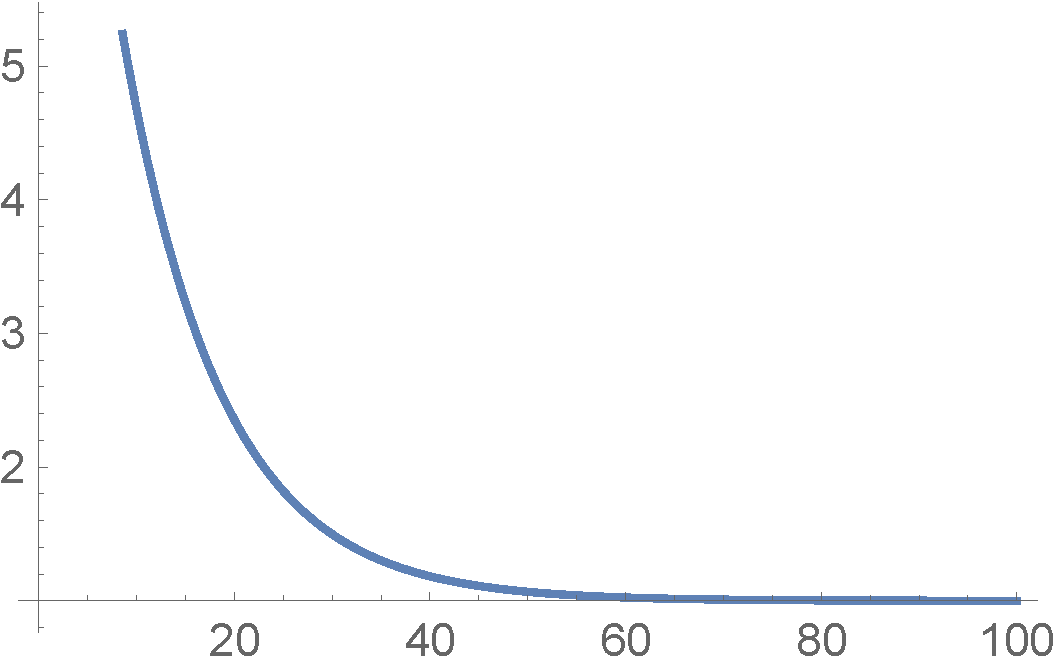
\includegraphics[width=0.5\textwidth]{脉冲放电图.pdf}
    \caption{脉冲放电图}
\end{figure} 

从而,当没有外部脉冲输入的情况下,膜电压会以指数形式衰减到$u_{rest}$。其衰减时间系数$\tau m$一般为10ms,与一般持续1ms的尖峰脉冲相比长了很多。
 
我们可以绘制对于方波输入,膜电压的变化图。我一开始打算利用解析解来绘制,但是发现分段条件太难设置了。因此我选择使用微分方程\ref*{微分方程}来模拟,这样子写成递归函数,会非常简便好看。代码和仿真图如下:\\

\begin{lstlisting}[language=Python]
def U(t_scale, tou, u_t_1, I, R, u_rest):
    return (-(u_t_1 - u_rest) + R*I)/tou*t_scale + u_t_1
\end{lstlisting}

\begin{figure}[H]
    \centering
    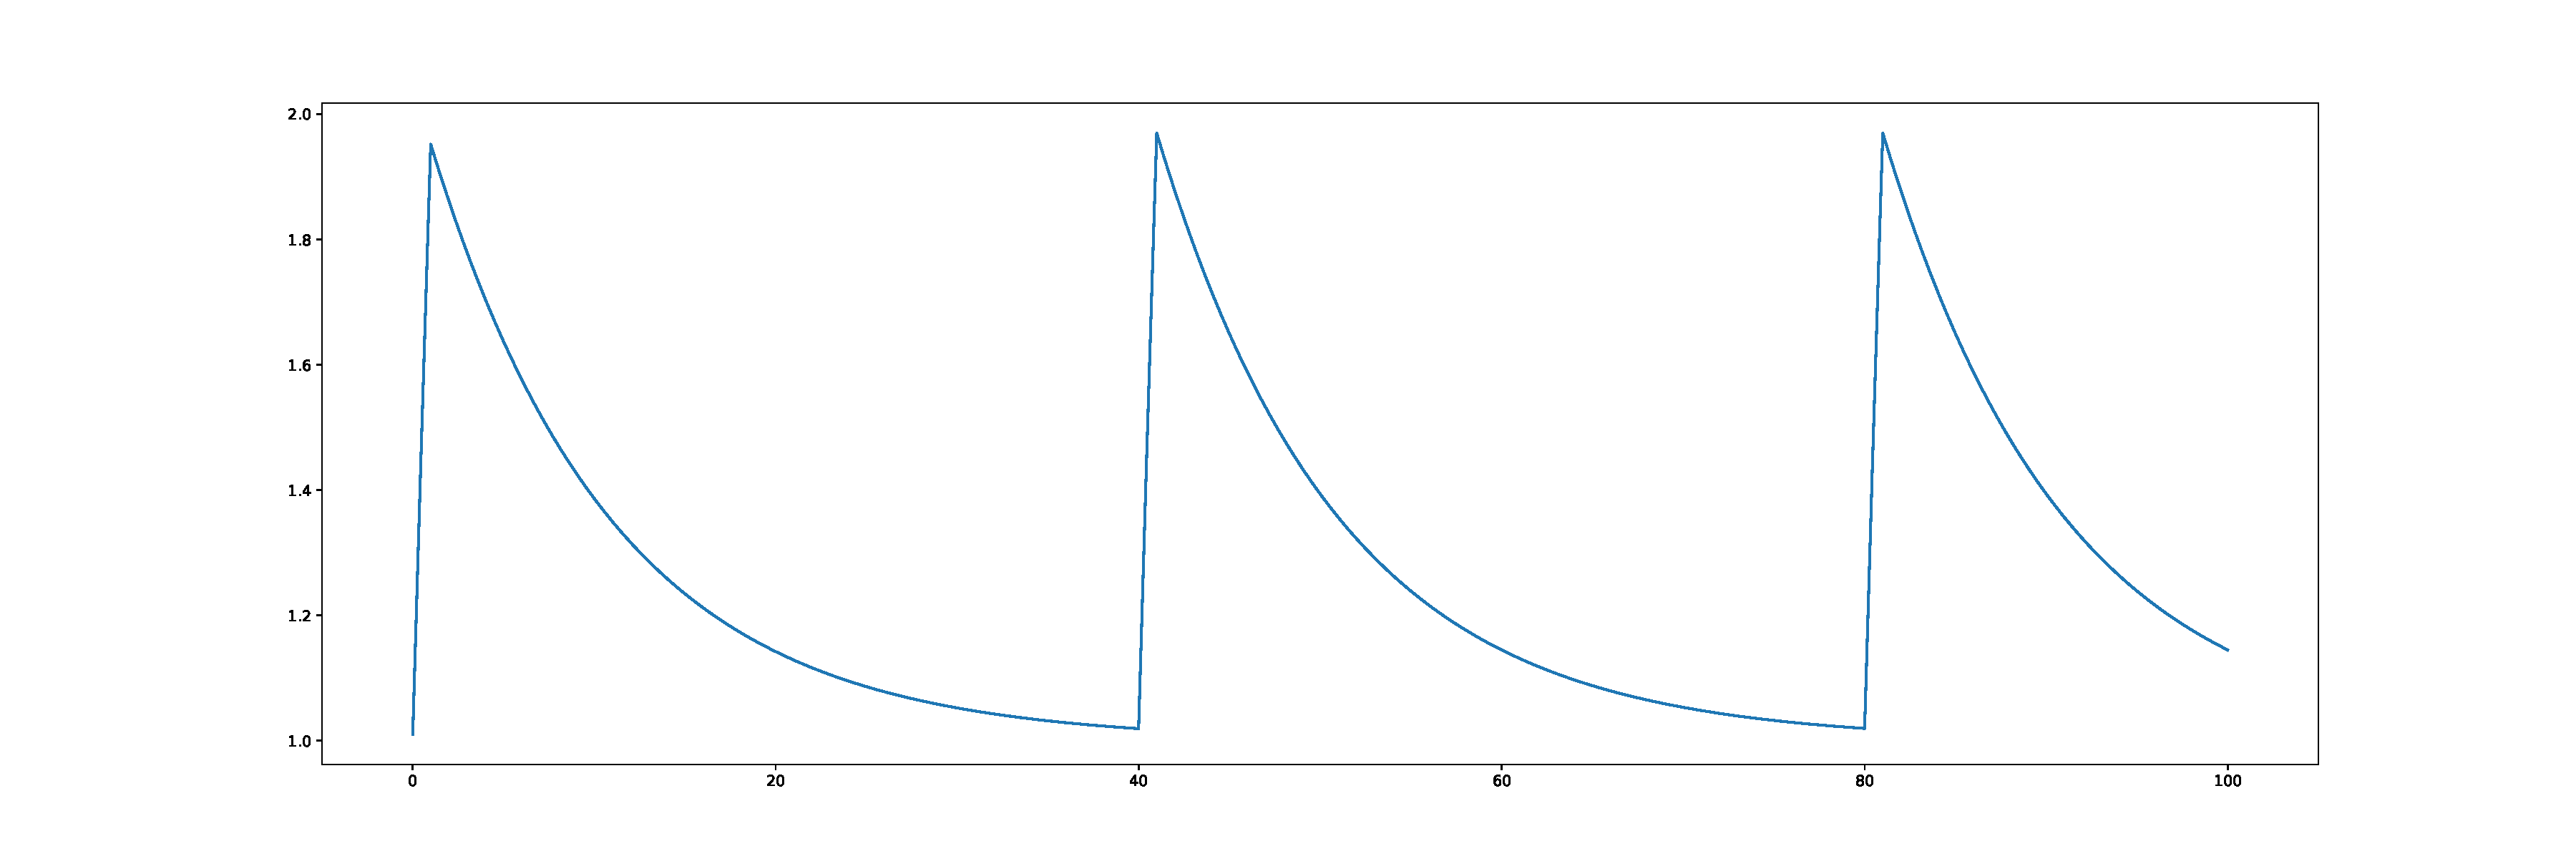
\includegraphics[width=1\textwidth]{方波输入响应图.pdf}
    \caption{方波输入响应图}
\end{figure} 

接下来,考虑输入电流I(t)为一个持续时间为$\Delta$的一个非常短的脉冲。其膜电压轨迹由\ref*{零状态响应}改写得:$u(\Delta)=u_{rest}+I_{max}R(1-e^{-\frac{\Delta}{\tau}})$。对e指数函数做泰勒展开,由于$\Delta$已经很小了,因此只需考虑其一阶情况即可:

\begin{equation}
    u(\Delta)=u_{rest}+I_{max}R\frac{\Delta}{\tau_m}\qquad for \Delta<<\tau_m
    \label{膜电压一阶泰勒}
\end{equation}

然后我们把$\Delta$推至无穷小,并I(t)变形为一个$\delta$函数。从而得到一个总电量$q=I_0\Delta$不变的脉冲。将$q=I_0\Delta$以及$\tau_m=RC$代入上式可得:

\begin{equation}
    u(\Delta)=u_{rest}+\frac{q}{C}
    \label{狄拉克函数}
\end{equation}

然后,可以得到输入脉冲结束后电压泄露到$u_{rest}$的过程。将上式带入\ref*{零输入响应},可得:

\begin{equation}
    u(t)=u_{rest}+\frac{q}{C}e^{-\frac{t-t_0}{\tau_m}}
    \label{脉冲响应}
\end{equation}

从而可以发现,非常窄电流脉冲输入等价于给细胞膜增加了一个$\frac{q}{C}$的电压。当膜电压高于阈值时,会发射一个脉冲,然后膜电压被重置为$u_{r}$,一定要注意,$u_{r}!=u_{rest}$,而是比$u_{rest}$要低一些。记在$t^f$时刻发射了脉冲。那么发射脉冲序列可以用狄拉克求和表示:

\begin{equation}
    S(t)=\sum \delta (t-t^f)
\end{equation}

前面\ref*{零状态响应}和\ref*{零输入响应}零状态响应和零输入响应描述的都是I(t)为恒定状态的情况。下面考虑I(t)为连续的变化信号的情况。由于离散的电流I输入实质上是给细胞膜引入一个$\Delta u=\frac{q}{C}=IR$的电压变化,因此连续变化的I(t)输入即公式\ref*{脉冲响应}与I(t)的卷积:

\begin{equation}
    \begin{aligned}
        u(t)&=u_{rest}+\frac{q}{C}e^{-\frac{t}{\tau_m}}\\
        &=u_{rest}+IRe^{-\frac{t}{\tau_m}}\\
        &=u_{rest}+RI(t)\bigotimes e^{-\frac{t}{\tau_m}}\\
        &=u_{rest}+R\int_0^{+\infty}I(t-s)e^{-\frac{s}{\tau_m}}d\frac{s}{\tau_m}\\
        &=u_{rest}+\frac{R}{\tau_m}\int_0^{+\infty}I(t-s)e^{-\frac{s}{\tau_m}}ds
    \end{aligned}
    \label{卷积}
\end{equation}

上面的式子相当于把输入电流分成无数多小的脉冲,每一个脉冲都会产生$\Delta ue^{-\frac{t}{\tau_m}}$的膜电压变化,然后全部积分起来。那么,同理,我们也可以用同样的方式描述发射脉冲的过程。发射一个脉冲,等价于膜上减少了$\vartheta -u_{r}$的电压,考虑到发射脉冲是离散的,因此我们可以表示为:

\begin{equation}
    \sum_f -(\vartheta -u_{r})e^{-\frac{t-t^f}{\tau_m}}
\end{equation}

因此,描述LF整个输入-输出的膜电压函数为:

\begin{equation}
    u(t)=u_{rest}+\sum_f -(\vartheta -u_{r})e^{-\frac{t-t^f}{\tau_m}}+\frac{R}{\tau_m}\int_0^{+\infty}I(t-s)e^{-\frac{s}{\tau_m}}ds
\end{equation}

\section{输入电流为周期性驱动及其傅里叶变换}

下面我们分析输入电流I(t)为周期性函数时,其膜电压响应的形式。我们定义$\kappa (s)=\frac{1}{C}e^{\frac{s}{\tau_m}}$,则输入电流引起的膜电压的响应可以写作:

\begin{equation}
    u(t)=\int_0^{+\infty}I(t-s)\kappa (s)ds
    \label{卷积公式}
\end{equation}

它具有很漂亮的滤波器的形式,可以看做是滤波器$\kappa(s)$对输入电流I(t)卷积。利用傅里叶变换(Fourier transform)可以得到其频域响应:

\begin{equation}
    u(\omega )=I(\omega )\kappa (\omega )
\end{equation}

现在我们考虑$I(t)=I_0e^{i\omega t}$,代入\ref*{卷积公式}可得:

\begin{equation}
    \begin{aligned}
        u(t)&=\int_0^{+\infty}\kappa (s)e^{-i\omega s}dsI_0e^{i\omega t}\\
        &=\kappa (\omega)I_0e^{i\omega t}
    \end{aligned}
\end{equation}

考虑$u(t)=u_0e^{i(\phi \kappa(\omega)+\omega t)}$,那么其实部增益就可以写作:

\begin{equation}
    \frac{u_0}{I_0}=|\kappa (\omega)|=\int_0^{+\infty}\kappa (s)e^{-i\omega s}ds=\frac{1}{C}|\frac{\tau_m}{1+i\omega \tau_m}|
\end{equation}

由于$\omega \tau_m\gg 1$,因此增益约等于$\frac{1}{C\omega}$。因此,其电压增益和输入频率成反比。下面我在python中试验一下嘿嘿。利用Brian2开源包构建LIF模型,频率从50Hz-500Hz,我们观察其spike的次数。可以看到,spike次数随频率增加有减少的趋势,一定程度上验证了上面的增益公式。

\begin{figure}[H]
    \centering
    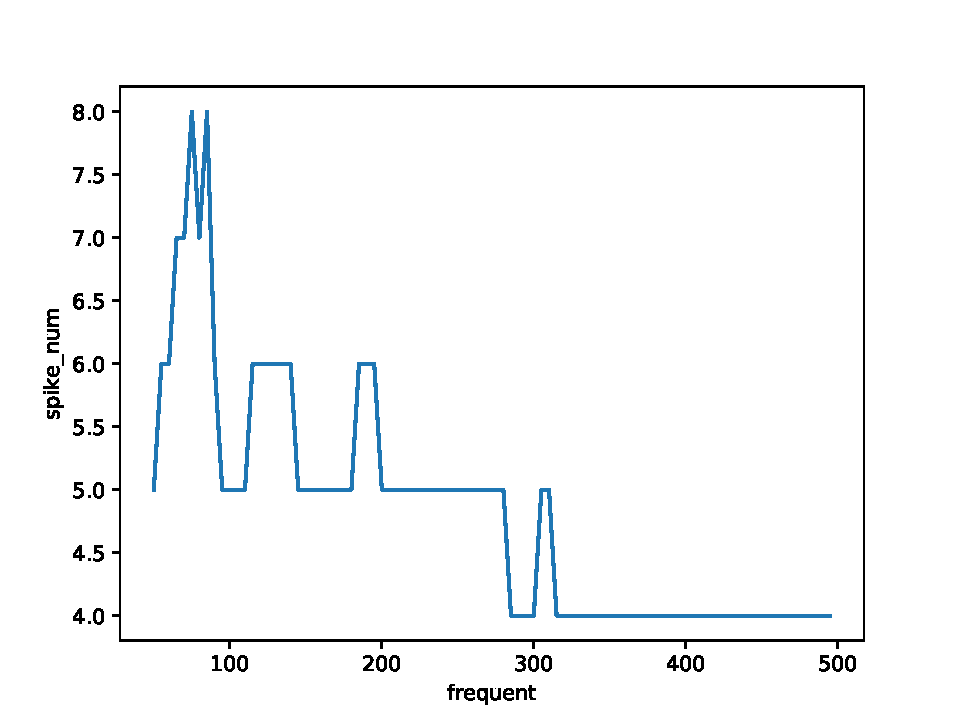
\includegraphics[width=0.5\textwidth]{增益和频率的关系.pdf}
    \caption{增益和频率的关系图}
\end{figure} 

\section{LIF模型的局限性}

我们介绍几种生物学上常见的神经元并以此阐述LIF模型的局限性。如下图所示:

\begin{figure}[H]
    \centering
    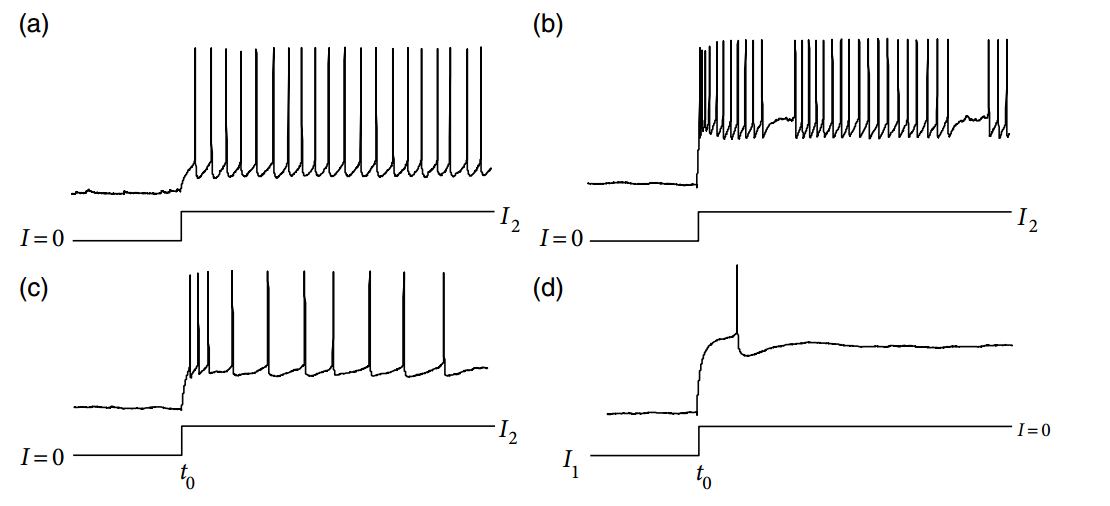
\includegraphics[width=1\textwidth]{四种神经元.png}
    \caption{四种神经元}
\end{figure}

图(a)所示就是LIF模型的神经元,对于一个持续的电流输入,由于神经元在每一次spike时都会重置为$u_{r}$,因此输出的spike序列是一个周期性的序列,这一类神经元也被称为\textbf{快速神经元(fast-spike neurons)}。图(b)所示的神经元叫做\textbf{突发口吃神经元(bursting and stuttering neurons)},它的特点是对于一个持续的电流输入,在一段时间内表现出周期性的输出,又非周期的出现一段长时间的不应期。图(c)所示的神经元叫做\textbf{适应性神经元(adaptation neurons)},与快速神经元不同,它具有适应性,它会积累输入的变化,在一段时间后变成稳定的脉冲输出。最后一种是\textbf{抑制后反弹神经元( post-inhibitory rebound neurons)},它会在输入停止后出现一个尖峰脉冲。上述的神经元在后面的章节中会做进一步讨论。

\section{总结}
由此,我们得到了神经元膜电压的积分方程,以及脉冲发射的方程。

\begin{equation}
    \begin{aligned}
        \tau _m\frac{du(t)}{dt}= -[u(t)-u_{rest}] + RI(t)\\
        \text{If}\quad u(t)=\vartheta \quad then \lim_{\delta \to 0;\delta>0} u(t+\delta)=u_r 
    \end{aligned}
\end{equation}

这个方程很简洁,也很好。但是在实际的神经元实验中,神经元会出现不应期(refractory)和适应性(adaptation)。不应期好处理。适应性考虑如下办法:每输出一个脉冲,给阈值$\vartheta$加一个小量,当输出脉冲为零(即静止状态时),阈值$\vartheta$衰减为初始值。仿照电路响应的微分方程,可以得到如下形式:公式中$\tau_{\text{adapt}}$为适应的时间常数,根据神经科学的实验,一般为几百毫秒。

\begin{equation}
    \tau_{\text{adapt}}\frac{\mathbf{d}}{\mathbf{d}t}\vartheta(t)=-[\vartheta(t)-\vartheta_0]+\theta\sum\limits_f\delta(t-t^f)
\end{equation}

\section{练习题}

\textbf{1、考虑突触输入电流为$\frac{q}{\tau_s}e^{-\frac{t-t_f}{\tau_s}}$($t>t_f$),$t_f$是电流到达突触的时间。}\\
\textbf{(a)求膜电压响应}\\\\
代入公式\ref*{卷积},求解其卷积响应即可。我的信号与系统有点忘光了,求了蛮久,响应如下(没化简):

\begin{equation}
    u(t)=u_{reset}+\frac{qR}{\tau_m-\tau_s}e^{-\frac{t-t_f}{\tau_s}}[e^{(t-t_f)(\frac{1}{\tau_s}-\frac{1}{\tau_m})}-1]
    \label{1.a的解}
\end{equation}

在mathematica文件\href{./exercise/exercise.nb}{exercise.nb}中验证了上式的正确性。并绘制了响应图

\begin{figure}[H]
    \centering
    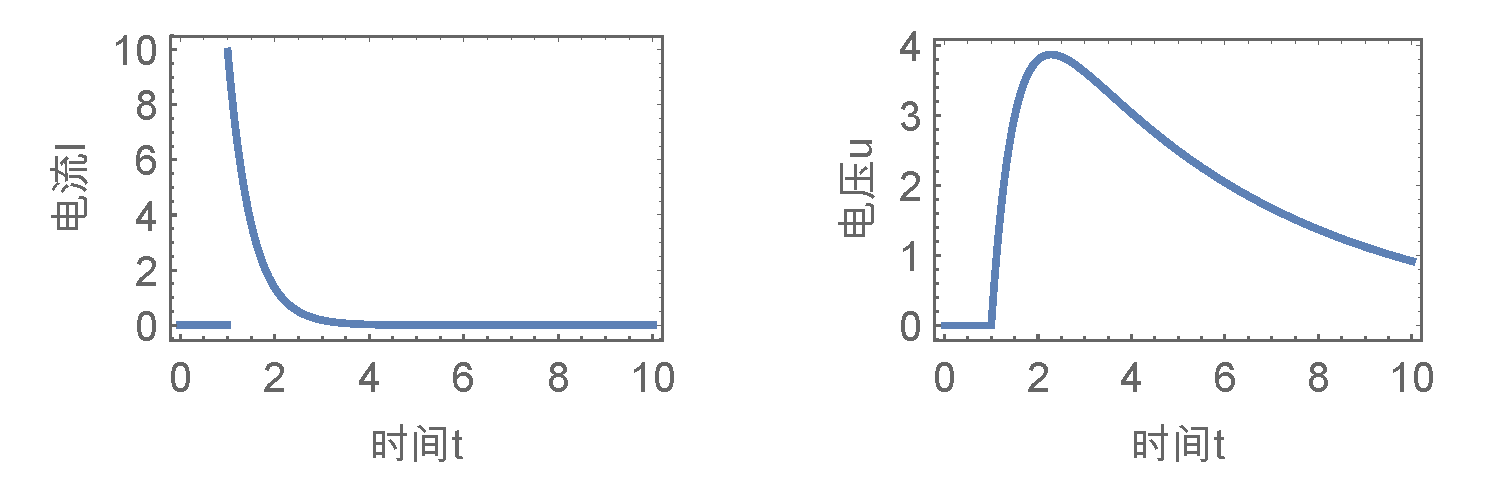
\includegraphics[width=1\textwidth]{exercise/1.a.pdf}
    \caption{1.apdf}
\end{figure}

\textbf{(b)在(a)的解中,取极限$\tau_s\to\tau_m$,并证明响应与$[t-t^{f}]\exp[-\frac{t-t^{f}}{\tau_\text{s}}]$成正比。这种形式的函数有时候被称为$\alpha$函数。}\\\\

显然,我们先计算如下部分:

\begin{equation}
    \begin{aligned}
        &\lim_{\tau_s\to\tau_m}=\frac{e^{(t-t_f)(\frac{1}{\tau_s}-\frac{1}{\tau_m})}-1}{\tau_s-\tau_m}\\
        &\text{利用等价无穷小}\\
        &=\lim_{\tau_s\to\tau_m}=\frac{(t-t_f)(\frac{1}{\tau_s}-\frac{1}{\tau_m})}{\tau_m-\tau_s}\\
        &=\frac{t-t_f}{\tau_m\tau_s}
    \end{aligned}
\end{equation}

代入公式\ref*{1.a的解},可得:

\begin{equation}
    u(t)=u_{reset}+\frac{qR}{\tau_m\tau_s}e^{-\frac{t-t_f}{\tau_s}}[t-t_f]
\end{equation}

从而可以证明,$u(t)$确实是与$[t-t^{f}]\exp[-\frac{t-t^{f}}{\tau_\text{s}}]$成正比的。

\textbf{(c)在(a)的解中,取极限$\tau_s\to0$。看看能不能把你的结论和狄拉克函数联系在一起?}\\\\

对公式\ref*{1.a的解}取极限,得:

\begin{equation}
    \begin{aligned}
        &\lim_{\tau_s\to0}u_{reset}+\frac{qR}{\tau_m-\tau_s}e^{-\frac{t-t_f}{\tau_s}}[e^{(t-t_f)(\frac{1}{\tau_s}-\frac{1}{\tau_m})}-1]\\
        &=\lim_{\tau_s\to0}u_{reset}+\frac{qR}{\tau_m-\tau_s}[e^{-\frac{t-t_f}{\tau_m}}-e^{-\frac{t-t_f}{\tau_s}}]\\
        &=u_{reset}+\frac{qR}{\tau_m}e^{-\frac{t-t_f}{\tau_m}}\qquad(t>t_f)
    \end{aligned}
\end{equation}

可以看到,当$\tau_s\to0$时,膜电压变化公式退化为公式\ref*{脉冲响应},即输入为狄拉克脉冲时的情形。同样,我们通过mathematica仿真一下。非常漂亮的一张图。

\begin{figure}[H]
    \centering
    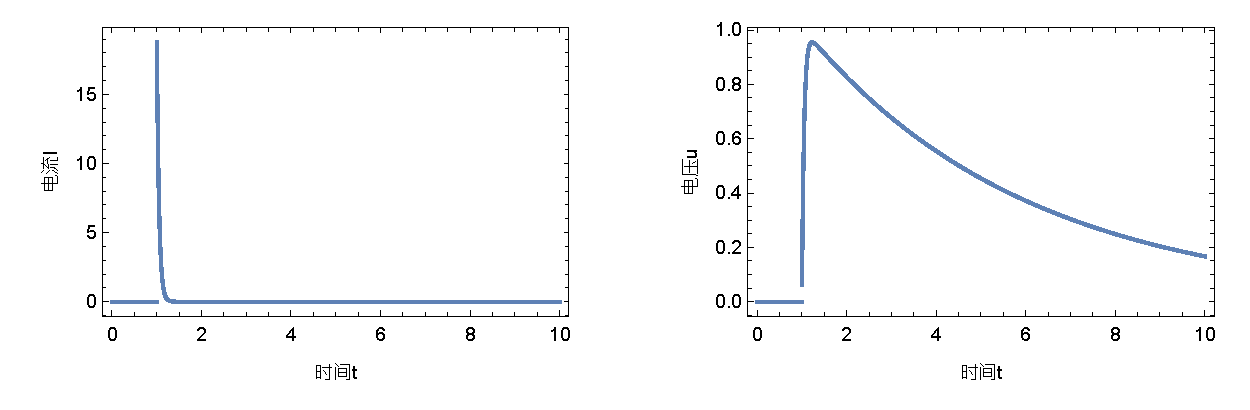
\includegraphics[width=1\textwidth]{exercise/1.c.pdf}
    \caption{1.cpdf}
\end{figure}

\textbf{2、考虑突触输入电流为随时间变化的电流输入(Time-dependent solution)。则可知其膜电压变化的解为公式\ref*{卷积}。现在我们交换公式\ref*{卷积}里卷积的顺序(卷积交换顺序不影响结果)。然后对该式求微分,比较一下微分方程两端的结果。}\\

这一段推导到了一上午。主要是高数的很多知识都忘记了。

\begin{equation}
    \begin{aligned}
        u(t)&=u_{rest}+\frac{R}{\tau_m}\int_0^\infty e^{-\frac{t-s}{\tau_m}}I(s)ds\\
        &\text{两边求导}\\
        \frac{du(t)}{dt}&=\frac{1}{dt}[u_{rest}+\frac{R}{\tau_m}\int_0^\infty e^{-\frac{t-s}{\tau_m}}I(s)ds]\\
    \end{aligned}
\end{equation}

这个地方踩了一个大坑,实际的积分上限是t,($t\to\infty$)区间没有意义,如果上限使用$\infty$,计算不出结果。

\begin{equation}
    \begin{aligned}
        \frac{du(t)}{dt}&=\frac{1}{dt}[u_{rest}+\frac{R}{\tau_m}\int_0^t e^{-\frac{t-s}{\tau_m}}I(s)ds]\\
        \frac{du(t)}{dt}&=\frac{1}{dt}[u_{rest}+\frac{R}{\tau_m}e^{-\frac{t}{\tau_m}}\int_0^t e^{\frac{s}{\tau_m}}I(s)ds]\\
    \end{aligned}
\end{equation}

这里链式积分和不定积分求导,应用$\Phi'(x)=\frac{d}{dx}\int_{\phi(x)}^{\varphi(x)}f(t)dt=f[\varphi(x)]\varphi'(x)-f[\phi(x)]\phi'(x)$

\begin{equation}
    \begin{aligned}
        \frac{du(t)}{dt}&=\frac{R}{\tau_m}\frac{-1}{\tau_m}[\int_0^t e^{-\frac{t-s}{\tau_m}}I(s)ds+\frac{R}{\tau_m}I(t)]\\
        \tau_m\frac{du(t)}{dt}&=-[u(t)-u_{rest}]+RI(t)\\
    \end{aligned}
\end{equation}

最终得到的形式和公式\ref*{微分方程}一致。这也正常,毕竟本身就是公式\ref*{微分方程}的一个解。

\textbf{3、假设在$t_f$时刻神经递质被传递到突触出,浓度为$\tau_x\frac{\text{d}x}{\text{d}t}=-x+\delta(t-t_f)$,神经递质与突触受体结合,打开离子通道,产生电流为$\tau_s\frac{\text{d}I}{\text{d}t}=-I+I_0x(t)$,并引起膜电压变化为$\tau_m\frac{\text{d}u}{\text{d}t}=-u+RI(t)$,求出膜电压变化公式。这三个传递构成了一个线性方程组(Chain of linear equations)}

对三条线性方程依次求解即可,我决定利用mathematica来求解,解得:

\begin{equation}
    x(t)=\frac{1}{\tau_x}e^{-\frac{t-t_f}{\tau_x}}\theta(t-t_f)
\end{equation}

\begin{equation}
    I(t)=\frac{I_0(e^{\frac{t_f-t}{\tau_s}}-e^{\frac{t_f-t}{\tau_x}})}{\tau_s-\tau_x}\theta (t-t_f)
\end{equation}

\begin{equation}
    \begin{aligned}
        u(t)&=I_0 R \theta (t-t_f) e^{-\frac{t}{\tau_m}-\frac{t}{\tau_s}-\frac{t}{\tau_x}}\\
        &(\tau_s (\tau_x-\tau_m) e^{\frac{t}{\tau_m}+\frac{t}{\tau_x}+\frac{t_f}{\tau_s}}+\\
        &\tau_m (\tau_s-\tau_x) e^{\frac{t}{\tau_s}+\frac{t}{\tau_x}+\frac{t_f}{\tau_m}}+\\
        &\tau_x (\tau_m-\tau_s) e^{\frac{t}{\tau_m}+\frac{t}{\tau_s}+\frac{t_f}{\tau_x}})\\
        &/((\tau_s-\tau_m) (\tau_m-\tau_x) (\tau_s-\tau_x))
    \end{aligned}
\end{equation}

具有某种规律性的美感。本章完结!

\chapter{离子通道和 Hodgkin–Huxley 模型}

Hodgkin–Huxley模型其等效电路图和LIF模型的区别是它考虑的钠离子和钾离子两个通道,并且给出了生物学上的具体意义。电路图如下所示:

\begin{figure}[H]
    \centering
    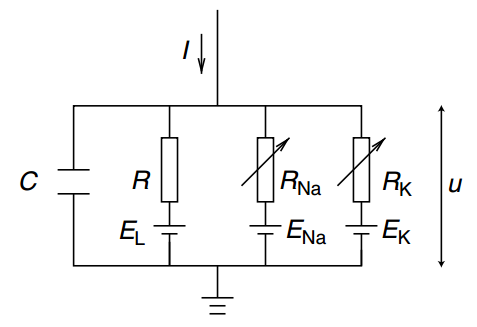
\includegraphics[width=0.7\textwidth]{HH模型电路图.png}
    \caption{HH模型电路图}
\end{figure}

它一共有3个支路,$R_{Na}、R_{K}$支路是钠离子、钾离子通道的等效电阻,$E_{Na}、E_{K}$是钠离子、钾离子的通道电势。这个电势是由离子浓度差引起的。它有一个专业名词叫能斯特电势(Nernst potential)。利用基尔霍夫定律,可以得到电路的微分方程如下:

\begin{equation}
    I(t)=I_C(t)+\sum_k I_k(t)
    I(t)=C\frac{du(t)}{dt}+g_{\text{Na}}(u-E_{\text{Na}})+g_{\text{K}}(u-E_{\text{K}})+g_{\text{L}}(u-E_{\text{L}})
    \label{HH微分方程}
\end{equation}

其中,$g_{\text{Na}}$和$g_{\text{K}}$是钠、钾通道的导纳。HH模型的主要工作也就是去测量拟合这个导纳。它表示为:

\begin{equation}
    \begin{aligned}
        g_{\text{Na}}&=\overline{g_{\text{Na}}}m^3h\\
        g_{\text{K}}&=\overline{g_{\text{K}}}n^4\\
        g_{\text{L}}&=\frac{1}{R}
    \end{aligned}
\end{equation}

$\overline{g_{\text{Na}}}$是钠离子通道的最大导纳,$\overline{g_{\text{K}}}$是钾离子通道的最大导纳。公式\ref*{HH微分方程}被写作:

\begin{equation}
    I(t)=C\frac{du(t)}{dt}+g_{\text{Na}}m^3h\left(u-E_{\text{Na}}\right)+g_{\text{K}}n^4\left(u-E_{\text{K}}\right)+g_{\text{L}}\left(u-E_{\text{L}}\right)
\end{equation}

其中m、n、h为某种离子通道打开的概率。每种通道类型激活的概率可以由激活和失活两部分叠加组成,其微分方程利用电压依赖性转换率$\alpha$和$\beta$来描述。

\begin{equation}
    \begin{aligned}
        \frac{dm}{dt}&=\alpha_m(u)(1-m)-\beta_m(u)m\\
        \frac{dn}{dt}&=\alpha_n(u)(1-n)-\beta_n(u)n\\
        \frac{dh}{dt}&=\alpha_h(u)(1-h)-\beta_h(u)h\\
    \end{aligned}
\end{equation}

$\alpha$和$\beta$是与当前膜电压相关的两组量,通过实验拟合为如下形式。\\

\begin{tabular}{ccc}
    \hline$x$ & $\alpha_x(u / \mathrm{mV})\left[\mathrm{ms}^{-1}\right]$ & $\beta_x(u / \mathrm{mV})\left[\mathrm{ms}^{-1}\right]$ \\
    \hline$n$ & $0.02(u-25) /\left[1-e^{-(u-25) / 9}\right]$ & $-0.002(u-25) /\left[1-e^{(u-25) / 9}\right]$ \\
    $m$ & $0.182(u+35) /\left[1-e^{-(u+35) / 9}\right]$ & $-0.124(u+35) /\left[1-e^{(u+35) / 9}\right]$ \\
    $h$ & $1 /\left[1+e^{-(u+62) / 6}\right]$ & $4 e^{(u+90) / 12} /\left[1+e^{-(u+62) / 6}\right]$ \\
    \hline
\end{tabular}

由此,HH模型就写完了。生物神经学有很多HH模型的变种,大概都是修改上面那个表格的拟合值。接下来用python模拟一下HH模型的神经元。

\section{输入方波激励}

我们给HH神经元输入一个方波电流激励,在文件\href{./python仿真代码/HH模型.py}{HH模型.py}利用brain2框架仿真模拟一下,跟踪了u,m,n,h的变化,如图所示。

\begin{figure}[H]
    \centering
    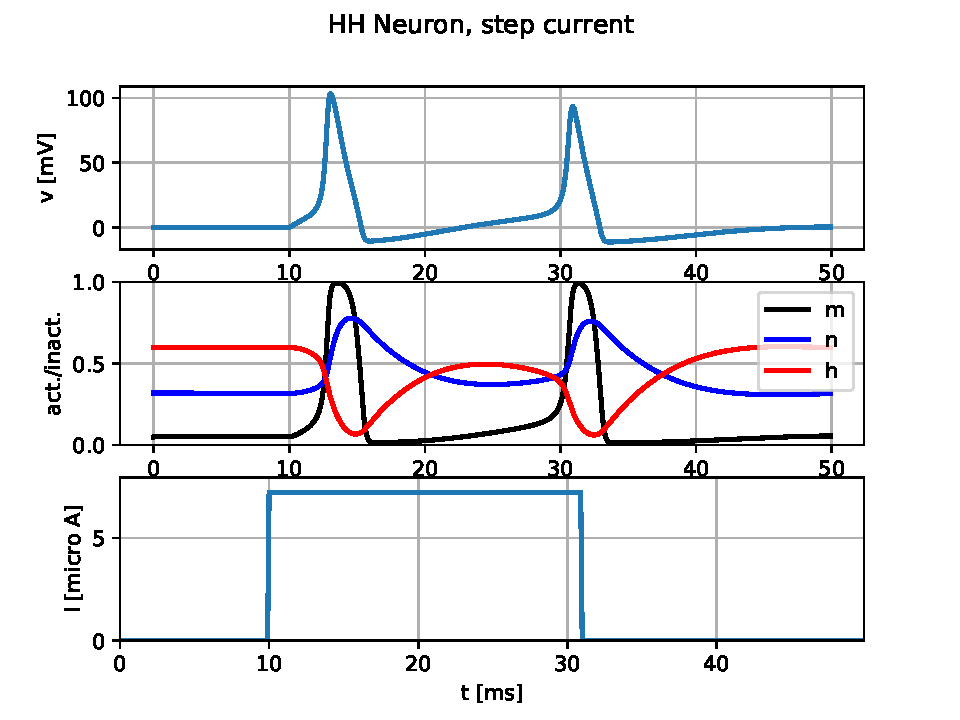
\includegraphics[width=0.7\textwidth]{HH模型方波激励.pdf}
    \caption{HH模型方波激励}
\end{figure}

由于这组线性微分方程太复杂了。因此我只能从仿真图去理解。

第一个阶段:可以看到当给入外加电流后,m,n,在快速上升,h在快速下降。m和h是控制钠离子通道开关的,由于m的时间常数比h的时间常数要大,因此结合在一起,钠离子通道是持续打开的,电荷内流。n控制钾离子通道,n变大控制钾离子通道打开,电荷外流。但是从图中的变化率可以看出,n,h的变化率都比m要慢,因此总的来说,电荷还是内流,从而使膜电压持续升高。

第二个阶段:当电压增加到一定程度,$dm/dt$反转变号时,m开始快速变小,由于n,h的时间常数比较大,具有电压感知滞后性,因此他们还在增大。从而导致钠离子通道开始快速关闭,钾离子通道还在打开。从而导致膜电压快速泄露。

第三个阶段:当$dn/dt$反转时,钾离子通道也开始缓慢关闭,电压泄露的速度减缓。

第四个阶段:$dh/dt$反转,电压泄露进一步减缓。由于n,h对电压感知滞后性,因此电压泄露到零时,还会进一步泄露,导致产生\textbf{过极化}。

第五个阶段,n,m,h会缓慢变化回初始值。观察图中两个脉冲后的恢复部分,可以发现,即便有外加电流的注入,这段恢复的过程也并没有很大的区别。因此,可以被称作不应期。

所以我对HH模型的直观理解是,它以连续的线性微分方程描述了在LIF模型中我们认为定义的\textbf{spike}和\textbf{不应期}两个东西。但是这微分方程确实很复杂,而且计算量也很大。我在brian2上仿真上面那张图,大概花了12秒。

定义\textbf{脉冲发射频率(fire rate)}为$v=\frac{1}{T}$,其中$T$是脉冲发射的时间间隔。由于脉冲发射频率是电流方波幅值$I_0$的函数,这个函数也被称为增益函数,我们可以画出增益函数来。

\begin{figure}[H]
    \centering
    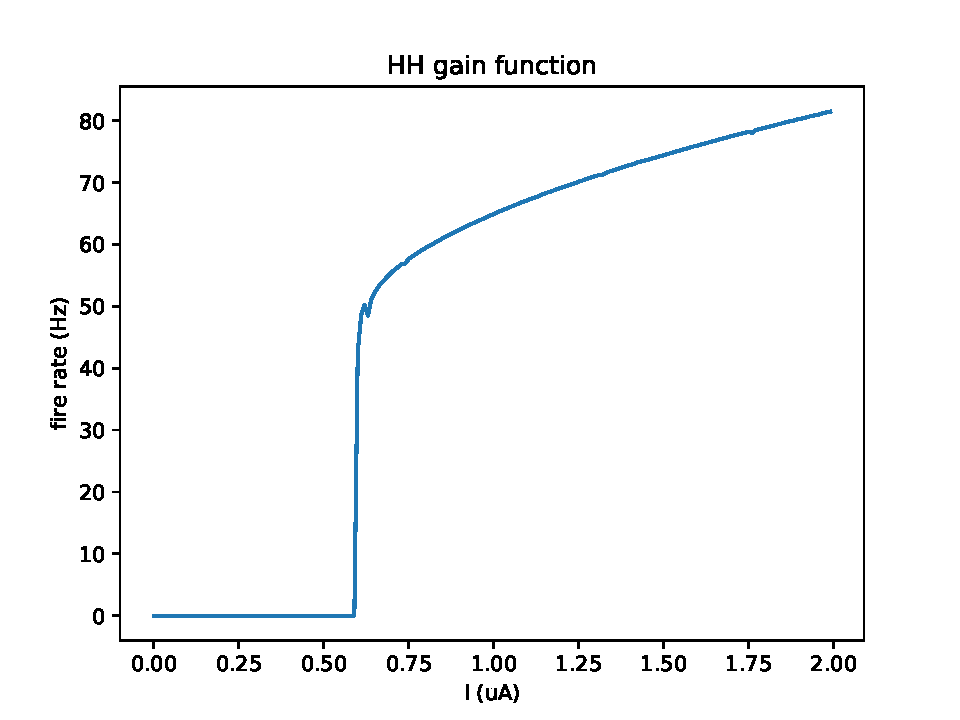
\includegraphics[width=0.5\textwidth]{HH增益函数.pdf}
    \caption{HH增益函数}
\end{figure}

可以看到,即便是连续的电流输入,它也是有电流幅值的阈值约束的,只有当幅值大于阈值,才能激发脉冲。而且它的fire rate是阶跃的,这种叫二型HH模型(type-\Rmnum{2})。通过调整模型的参数,可以得到fire rate是连续的模型,称为一型HH模型(type-\Rmnum{1})。

\section{总结}

HH模型从生物物理的角度解释了神经元的原理。其仿真结果与实际的生物的神经元电信号结果非常吻合。但是在后面的章节,还是会利用第一章讲的广义LIF模型去构建网络。所以这一章HH模型就是作为了解,作为其生物物理背景得补充。

\chapter{降维及相平面分析}

HH模型很好的契合了生物模型。但是4个微分方程组成的微分方程组是难以使用计算机去计算模拟的,因此我们需要对它进行降维。具体的做法是:由于m参数变化速率很快,因此可以将其看作是一瞬间就完成了的,作为一个常数,而n,h参数具有同样的变化特性,因此拟合为一个描述恢复的微分方程,加上膜电压u的那个微分方程,一共两个维度。从而将4维降到了两维。具体由两个模型给出。

\section{FitzHugh-Nagumo模型}
\textcolor[rgb]{1,0,0}{本小节仿真代码链接:\href{./降维到二维/FitzHugh-Nagumo模型.nb}{FitzHugh-Nagumo模型.nb}}\\
FitzHugh-Nagumo模型是最早提出的HH简化模型,它成功的描述了神经元的发射特性。它表示为如下形式:

\begin{equation}
    \begin{aligned}
        \frac{du}{dt}&=u-\frac{1}{3}u^3-w+I\\
        \frac{dw}{dt}&=\epsilon(b_0+b_1 u-w)
    \end{aligned}
\end{equation}

第一条式子描述的是膜电压的充电过程,第二条式子描述的是恢复过程,w是表征恢复的变量。这是一个很简单的线性系统,然而神奇的是它能很好的表征发射过程。接下来我们利用相图分析法(phase analysis)来分析它的变化过程。这个系统,u和w都在随t而变化,将u和w的变化趋势投影到u-w平面,就能得到其相图,如下图所示。图中箭头是变化趋势,我们绘制du/dt为0的曲线以及dw/dt为零的线,他们称为零斜率线(nullclines),如图中绿线及黄线所示。他们有一个交点,称为平衡点。红线是初始值为(-2,0.5)的点的运动轨迹,可以看到是向平衡点靠拢的。图(b)是对应的电压变化图,并不会产生脉冲发射。

\begin{figure}[H]
    \centering
    \subfigure[相图]{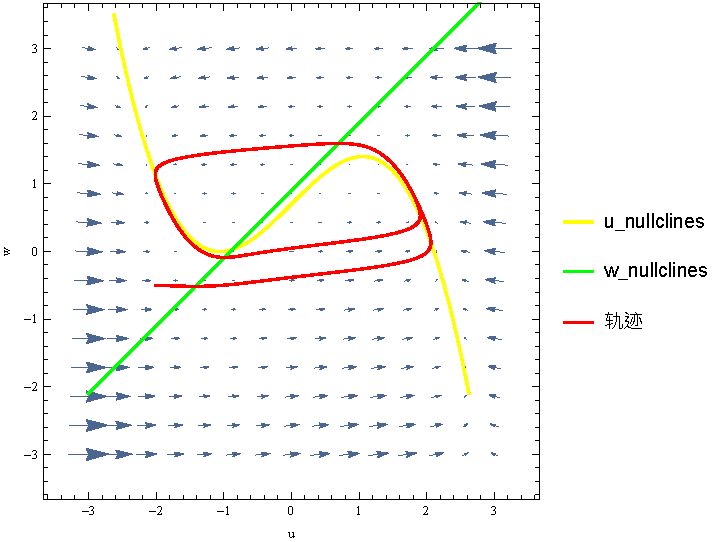
\includegraphics[width=0.4\textwidth]{降维到二维/Is=0FN相图.pdf}}
    \subfigure[电压变化图]{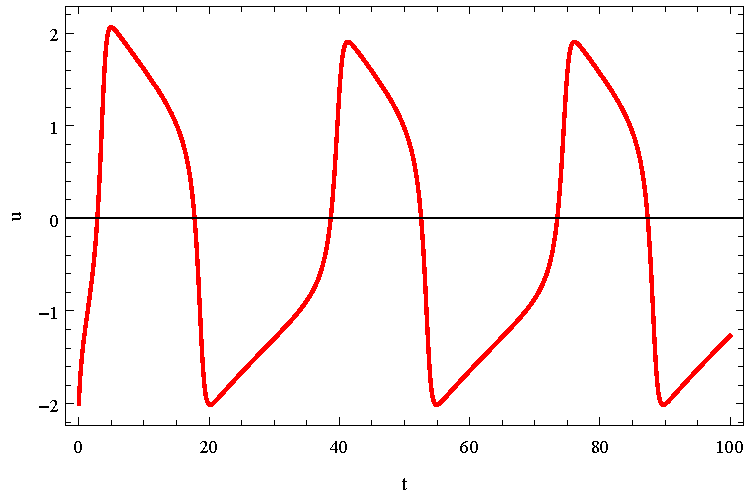
\includegraphics[width=0.4\textwidth]{降维到二维/Is=0FN电压.pdf}}
    \caption{Is=0时,FN模型}
\end{figure}

随着输入电流的增大,$u_{nullclines}$曲线会向上平移,平衡点的位置也会改变。现在我们定量的分析一下平衡点。记平衡点为$u_{ncs}$,$w_{ncs}$,我们需要分析平衡点周围的一个邻域的变化趋势。做如下变量替换:$n=u-u_{ncs}$,$v=w-w_{ncs}$,记原微分方程组为:$\frac{du}{dt}=F(u,w)$,$\frac{dw}{dt}=G(u,w)$,可得$\frac{dn}{dt}=F(n+u_{ncs},v+w_{ncs})$,$\frac{dv}{dt}=G(n+u_{ncs},v+w_{ncs})$。然后我们求取二阶偏导,得到导数的变化趋势,即:

\begin{equation}
    \begin{aligned}
        \frac{d^2n}{dt^2}&=\frac{\partial F(n+u_{ncs},v+w_{ncs})}{\partial n}\frac{\partial n}{\partial t}+\frac{\partial G(n+u_{ncs},v+w_{ncs})}{\partial n}\frac{\partial v}{\partial t}\\
        &=F_nF(n+u_{ncs},v+w_{ncs})+G_nG(n+u_{ncs},v+w_{ncs})\\
        \frac{d^2v}{dt^2}&=\frac{\partial F(n+u_{ncs},v+w_{ncs})}{\partial v}\frac{\partial v}{\partial t}+\frac{\partial G(n+u_{ncs},v+w_{ncs})}{\partial v}\frac{\partial v}{\partial t}\\
        &=F_vF(n+u_{ncs},v+w_{ncs})+G_vG(n+u_{ncs},v+w_{ncs})
    \end{aligned}
\end{equation}

上式可以被写作矩阵的形式:

\begin{equation}
    \frac{d}{dt}
    \begin{pmatrix}
        F(n+u_{ncs},v+w_{ncs})\\
        G(n+u_{ncs},v+w_{ncs})
    \end{pmatrix}
    =
    \begin{pmatrix}
        F_n & G_n\\
        F_v & G_v
    \end{pmatrix}
    \begin{pmatrix}
        F(n+u_{ncs},v+w_{ncs})\\
        G(n+u_{ncs},v+w_{ncs})
    \end{pmatrix}
\end{equation}

求解上式的特征值$\lambda_1$和$\lambda_2$,其中有6种情况,具体可见\href{https://zhuanlan.zhihu.com/p/141475551}{[非线性系统,平衡点稳定性]}:\\
1、当$\lambda_1<\lambda_2<0$时,为稳定点(Stable Node)。\\
2、当$\lambda_1>\lambda_2>0$时,为不稳定点(Unstable Node)。\\
3、当$\lambda_1>0>\lambda_2$时,为鞍点(Saddle)。\\
4、当$\lambda_{1,2}=\alpha+j\beta,\alpha>0$,为不稳定焦点(Unstable Focus)。\\
5、当$\lambda_{1,2}=\alpha+j\beta,\alpha=0$,为中心点(Center)。\\
6、当$\lambda_{1,2}=\alpha+j\beta,\alpha<0$,为稳定焦点(Stable Focus)。\\

当我们将电流逐渐增大时,求解的特征值也在发生变化。当$I\leqslant0.1mA$时,平衡点为稳定点;当$0.1mA<I\leqslant0.59mA$时,平衡点为稳定焦点;当$0.59mA<I$时,平衡点为不稳定焦点,此时开始周期震荡并发射脉冲,如下图所示。

\begin{figure}[H]
    \centering
    \subfigure[相图]{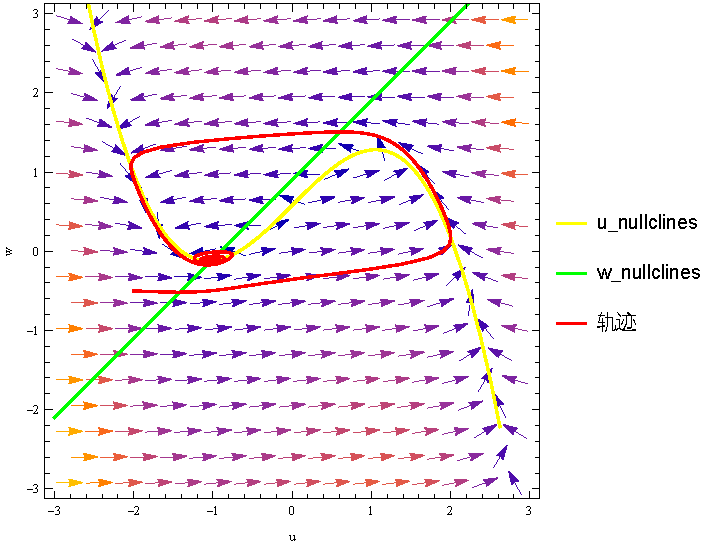
\includegraphics[width=0.4\textwidth]{降维到二维/Is=58FN相图.pdf}}
    \subfigure[电压变化图]{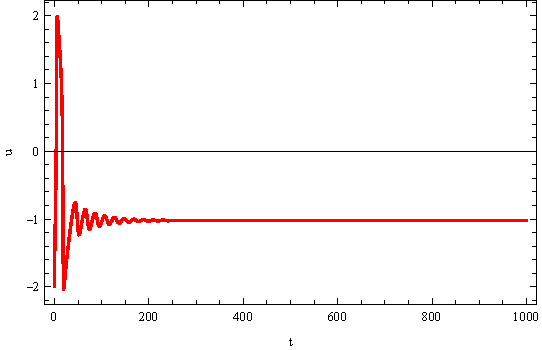
\includegraphics[width=0.4\textwidth]{降维到二维/Is=58FN电压.pdf}}
    \caption{Is=58时,FN模型}
\end{figure}

\begin{figure}[H]
    \centering
    \subfigure[相图]{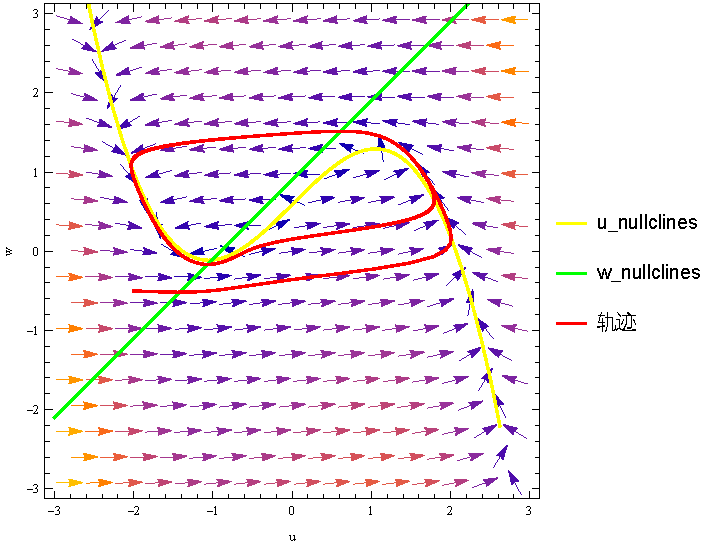
\includegraphics[width=0.4\textwidth]{降维到二维/Is=59FN相图.pdf}}
    \subfigure[电压变化图]{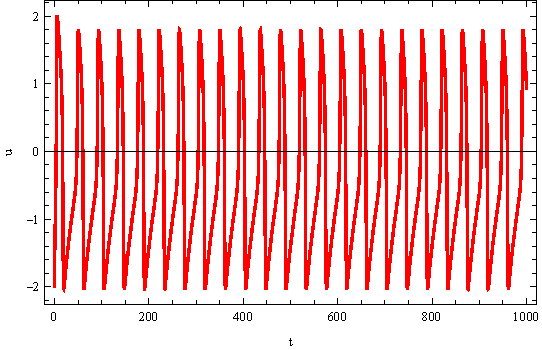
\includegraphics[width=0.4\textwidth]{降维到二维/Is=59FN电压.pdf}}
    \caption{Is=59时,FN模型}
\end{figure}

\text{真酷~~~~~~~~~~~~~}

\section{Morris-Lecar模型}
\textcolor[rgb]{1,0,0}{本小节仿真代码链接:\href{./降维到二维/Morris-Lecar模型.nb}{Morris-Lecar模型.nb}}\\
下面讨论一个更cool的模型。这个模型可以模拟第二章中讨论的细胞发射脉冲的I型和II型的情况。它的微分方程如下:

\begin{equation}
    \begin{aligned}
        C_m\frac{du}{dt}&=-g_k n (u-E_k)-g_l (u-E_l)-g_{na} m_\infty (u-E_{na})+I\\
        \frac{dn}{dt}&=\phi  (n_\infty-n)\\
        m_\infty&=0.5 (1+\tanh(\frac{u-u_1}{u_2}))\\
        n_\infty&=0.5 (1+\tanh(\frac{u-u_3}{u_4}))\\
        \phi &=0.1 \cosh (\frac{u-u_3}{2 u_4})
    \end{aligned}
\end{equation}

这个模型也是简化的HH模型,同样,我们绘制它的相图,研究它的动力学原理。可以看到,$u_{nullclines}$和$n_{nullclines}$存在三个平衡点。通过计算特征值,可以知道,最左边的一个平衡点是稳定结点(node),中间的平衡点是鞍点(saddle),最右边的平衡点是不稳定焦点。它和FitzHugh-Nagumo模型的分析差不多,当输入电流增大时,$u_{nullclines}$向上平移,左边的两个平衡点融合消失,整个模型开始在最右边的不稳定焦点处循环震荡,称为极限环(limit cycle),激发周期性脉冲。

\begin{figure}[H]
    \centering
    \subfigure[相图]{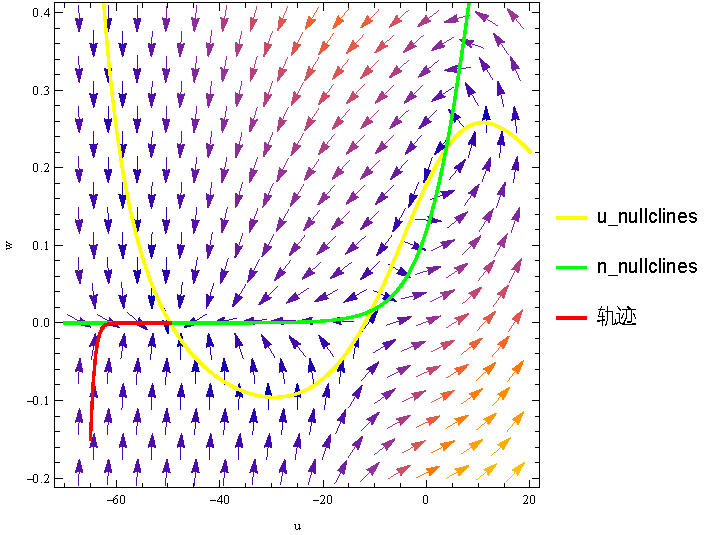
\includegraphics[width=0.4\textwidth]{降维到二维/Is=0ML相图.pdf}}
    \subfigure[电压变化图]{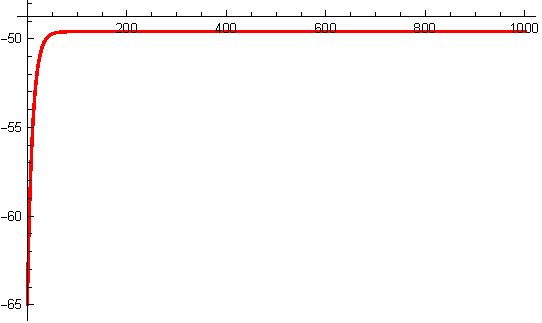
\includegraphics[width=0.4\textwidth]{降维到二维/Is=0ML电压.pdf}}
    \caption{Is=0时,ML模型}
\end{figure}

但是,极限环经过左边两个平衡点的不同位置却会导致两种不同的情况。当极限环经过结点转向鞍点时,尽管结点已经消失,但它所处的那片区域的速率依然非常低,因此脉冲激发的周期非常大,随着输入电流的增大,脉冲激发的周期逐渐减小,从而形成了I型的情况,即电流越过阈值后,脉冲激发速率从零开始变化,称为鞍结分叉型(saddle-node bifurcation),如下图所示:

\begin{figure}[H]
    \centering
    \subfigure[相图]{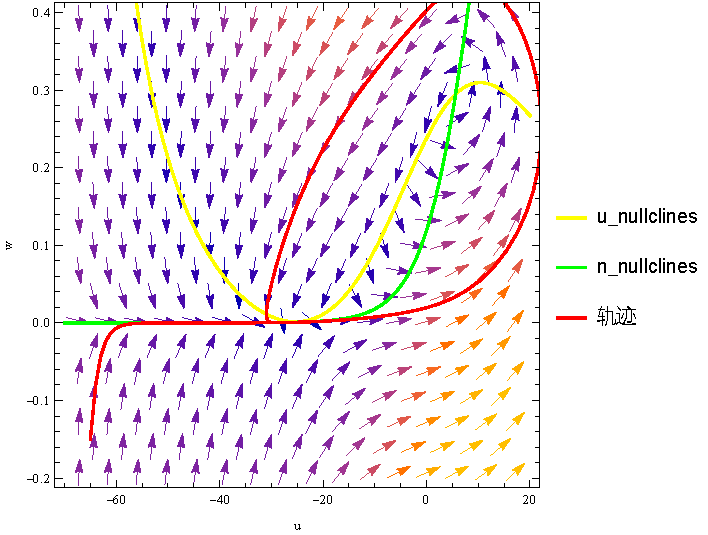
\includegraphics[width=0.4\textwidth]{降维到二维/Is=33.3ML鞍结分叉相图.pdf}}
    \subfigure[电压变化图]{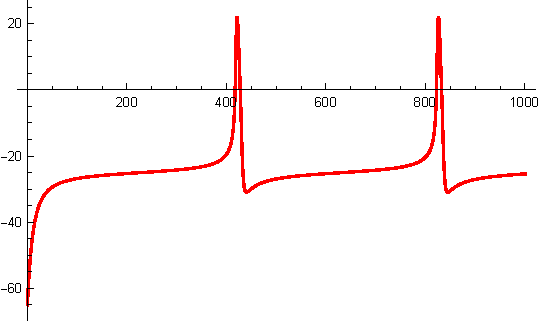
\includegraphics[width=0.4\textwidth]{降维到二维/Is=33.3ML鞍结分叉电压.pdf}}
    \caption{Is=33.3时,ML鞍结分叉模型(u4=10)}
\end{figure}

另一种是,极限环不经过结点,在鞍点的右侧划过,当电流超过阈值,产生极限环后,脉冲激发的速率从0阶跃到了一个较快的频率,从而形成二型的情况,称为Hopf分叉(Hopf bifurcation),如下图所示:

\begin{figure}[H]
    \centering
    \subfigure[相图]{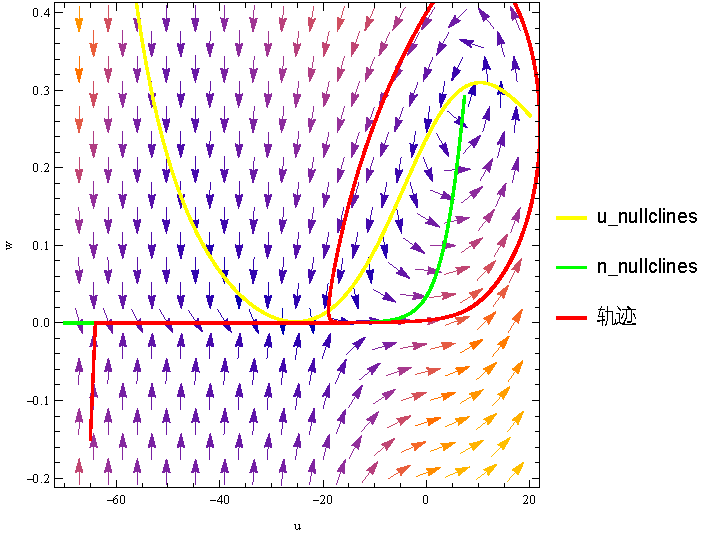
\includegraphics[width=0.4\textwidth]{降维到二维/Is=33.3MLHopf分叉相图.pdf}}
    \subfigure[电压变化图]{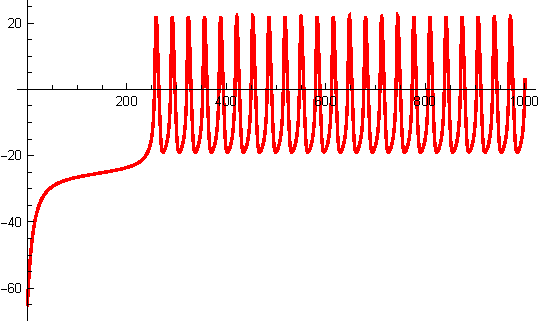
\includegraphics[width=0.4\textwidth]{降维到二维/Is=33.3MLHopf分叉电压.pdf}}
    \caption{Is=33.3时,ML鞍结分叉模型(u4=6)}
\end{figure}

OK,这一章把HH模型简化到二维。后面还对脉冲输入和连续输入做了讨论,就不表了,准备跳到第五章去。第五章开始第二部分,就要进一步简化HH模型为一维,讨论广义的非线性IF模型了。

\end{document}

